\section{Supplementary Material}

Gene functions are overlapping in several biological categories.
To better understand the reason why many pathways associated with diseases emerge in the results despite not all of them are associated with cancer.
To that end we tried to assess wheter genes that were associated with biological functions that are often deregulated in cancer were also present in pathways associated to dieases.
Figures \ref*{supp:gene-contrib-kegg-tcga} and \ref*{supp:gene-contrib-reactome-tcga} shows that genes are raely associated to one pathway and one biological category only in both Reactome and KEGG.
In KEGG, genes involved in \textit{Genetic Information Processing} or in \textit{Cellular Processes} are also involved in pathways linked to diseases.
In addition, some of these genes are also upregulated in 90\% of the samples.
\begin{figure}[h]
    \centering
    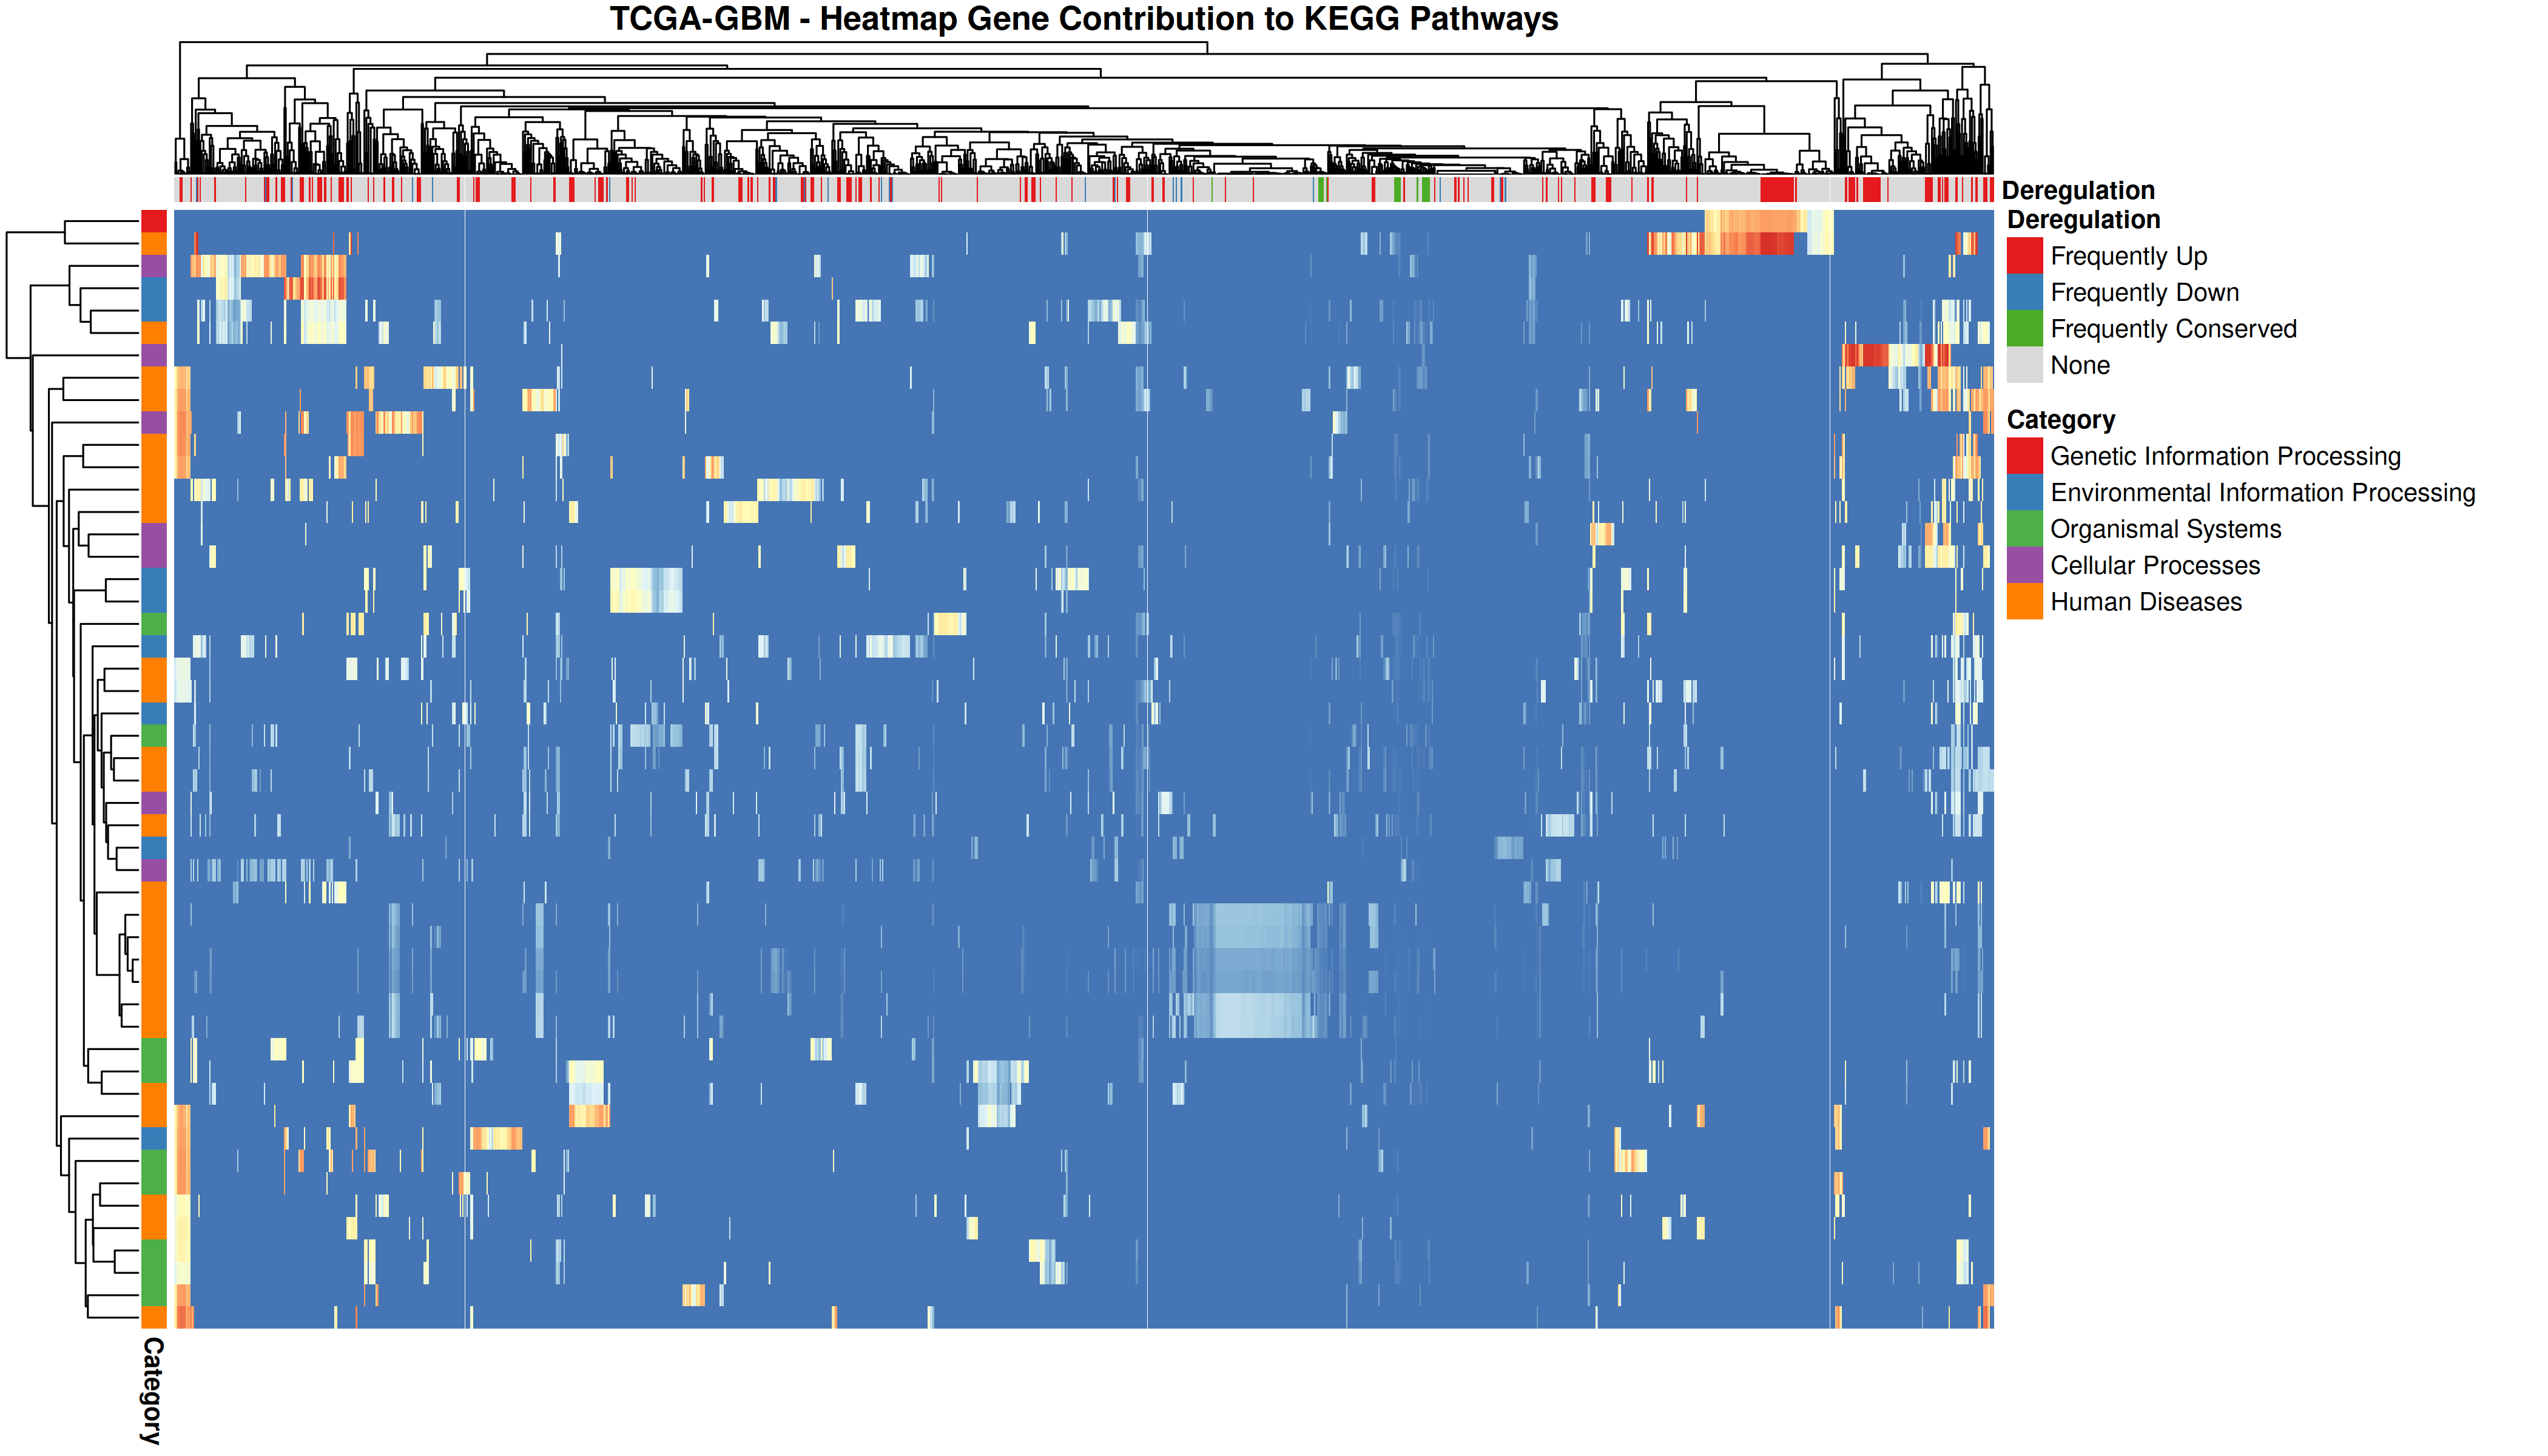
\includegraphics[width=\textwidth]{img/gene_contrib_kegg_tcga}
    \caption {
        Heatmap of the gene contributions for each pathways with \acrshort{tcga} data and \acrshort{kegg} categories.
        Genes contribution to a pathway is computed by calculating how many times a gene appear in the enrichment result for a pathway.
        Red colour indicates a strong contribution and blue colour indicates a week contribution.
        Only genes with a total contributions higher than the third quartile and pathways where the total gene contribution is higher than the third quartile are kept.
        Pathways are colored by their categories.
        Genes are colored by their deregulation frequency : red indicates genes that are up-regulated in 90\% of the samples, blue indicates genes that are down-regulated in 90\% of the samples, green indicates genes that are not deregulated in 90\% of the samples and grey genes that correspond to none of the above.
    }
    \label{supp:gene-contrib-kegg-tcga}

\end{figure}
In Reactome, we see that genes that are involved in the \textit{Extracellular Matrix Organization} and in the \textit{Metabolism of proteins} are also involed in pathways linked to diseases.
Like for KEGG, some are upregulated in 90\% of the samples as well.
\begin{figure}[h]
    \centering
    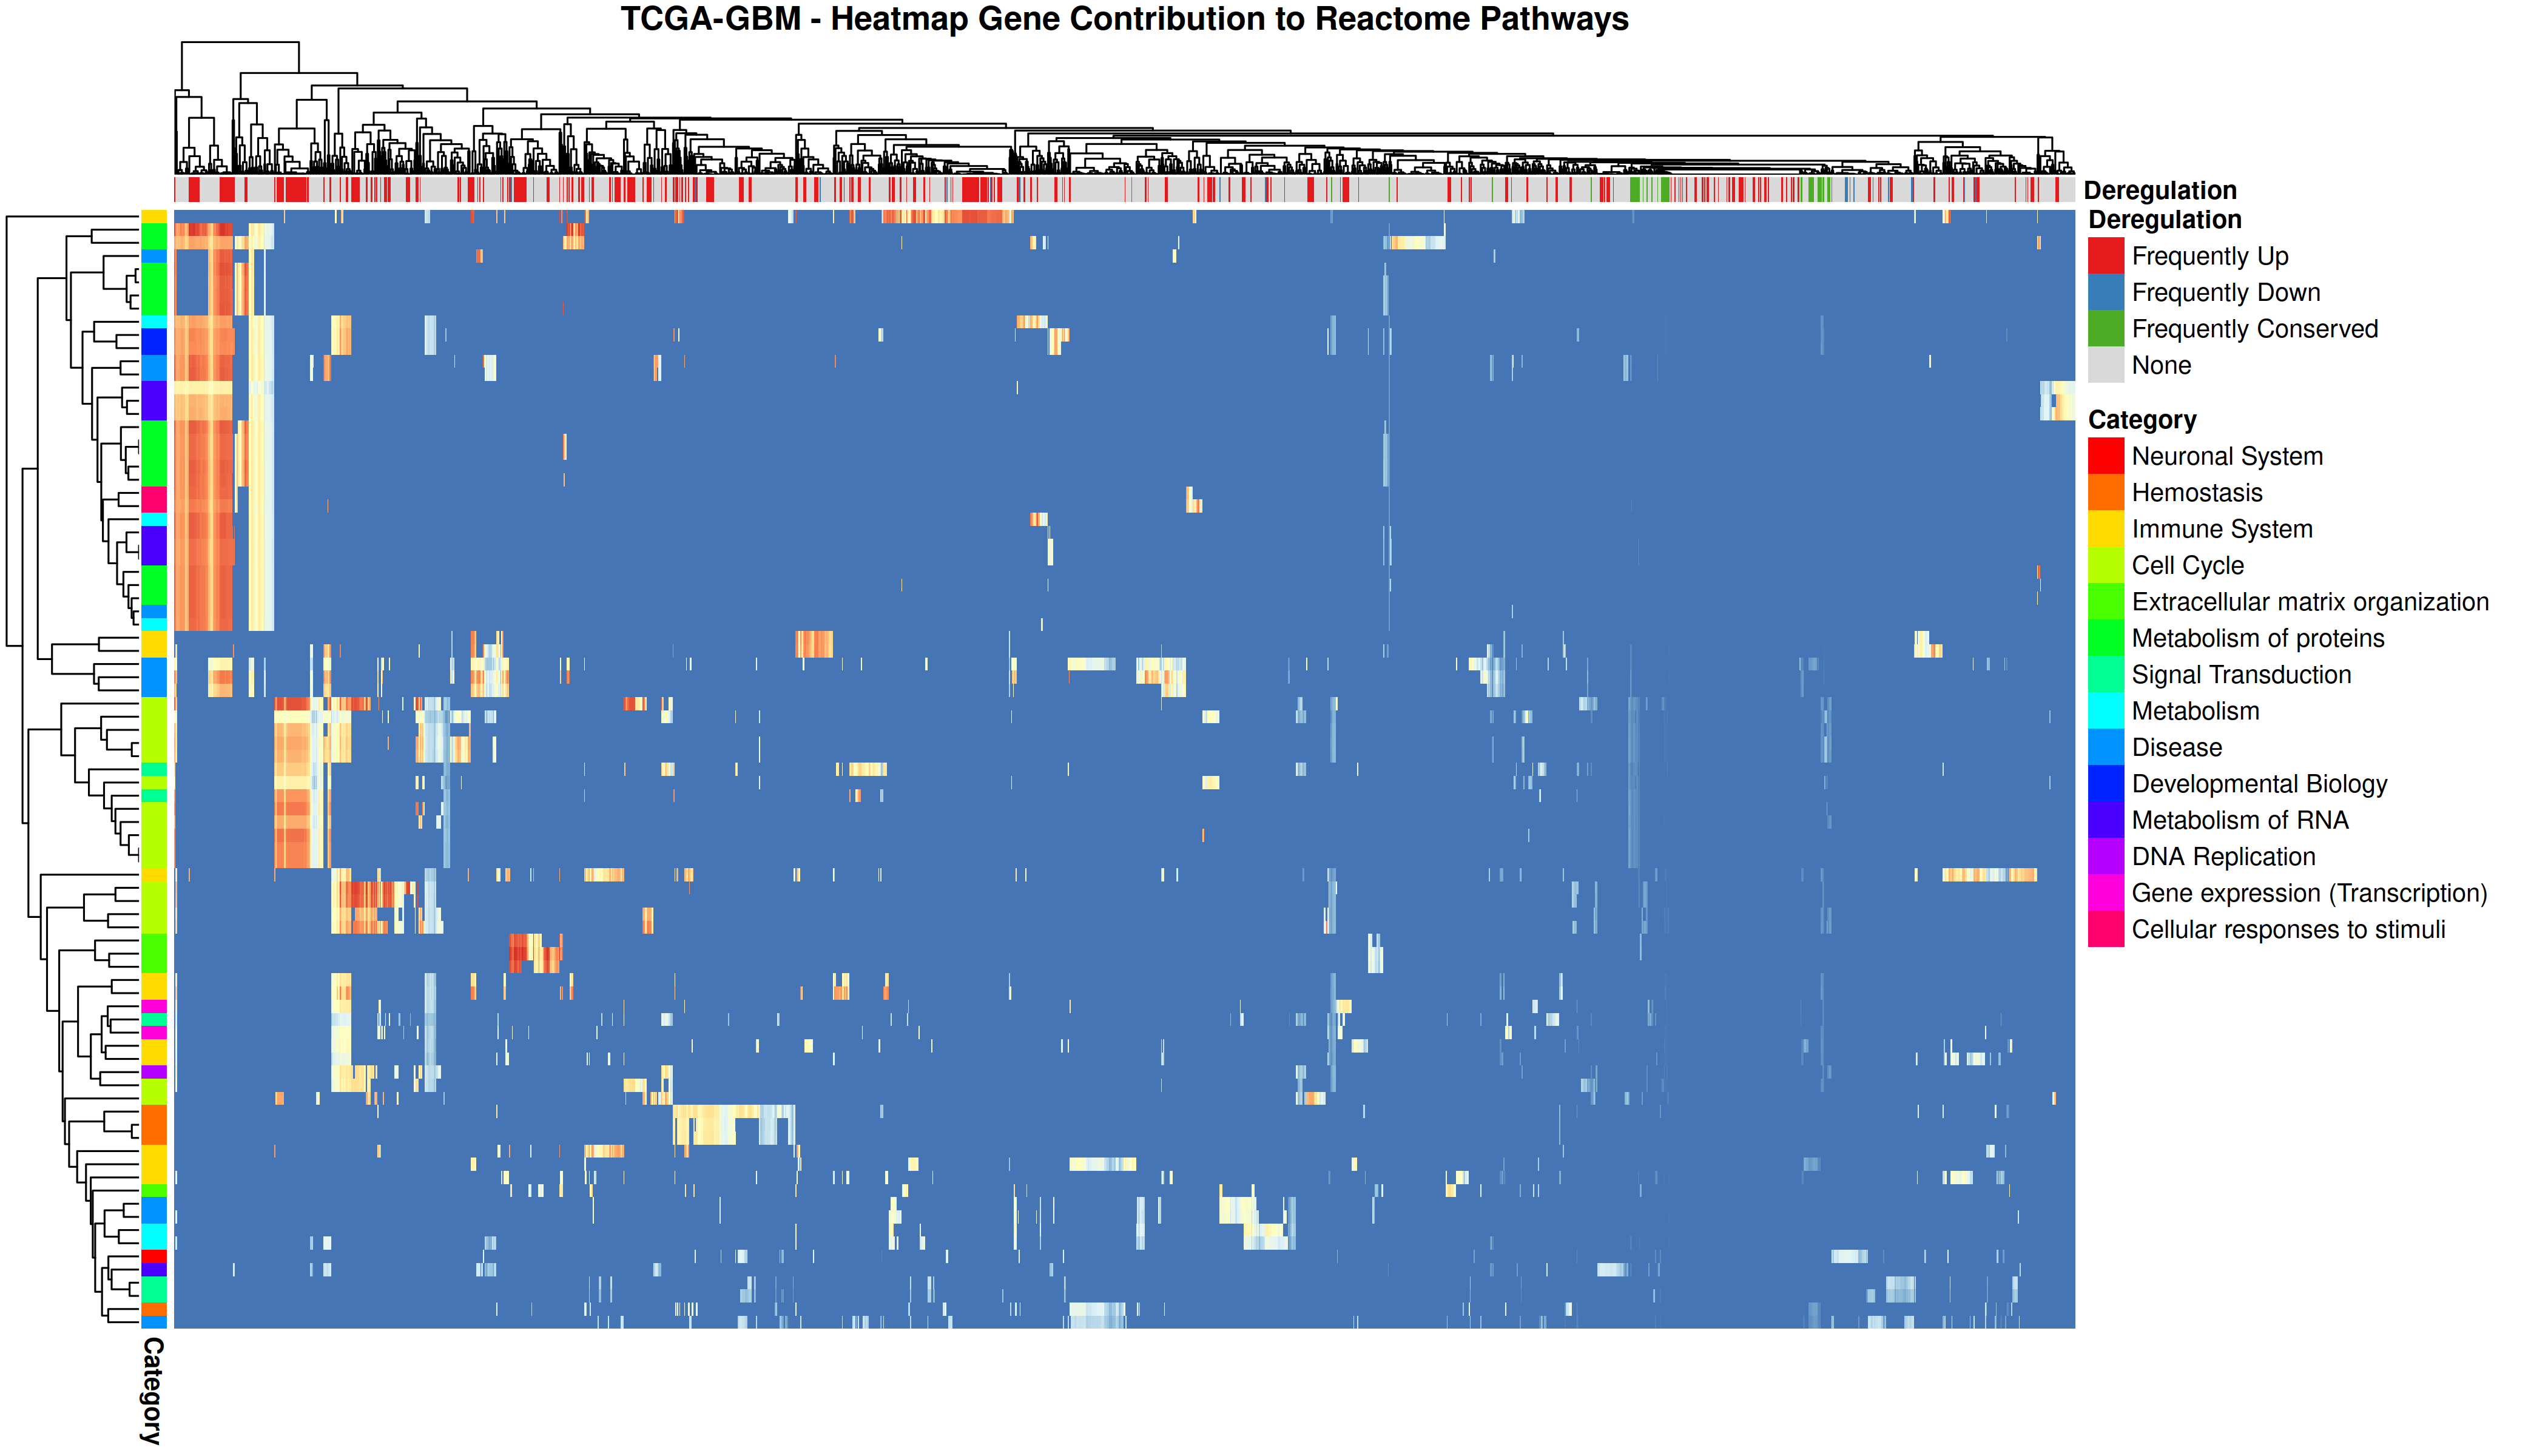
\includegraphics[width=\textwidth]{img/gene_contrib_reactome_tcga}
    \caption {
        Heatmap of the gene contributions for each pathways with \acrshort{tcga} data and Reactome categories.
        Genes contribution to a pathway is computed by calculating how many times a gene appear in the enrichment result for a pathway.
        Red colour indicates a strong contribution and blue colour indicates a week contribution.
        Only genes with a total contributions higher than the 90\% percentile and pathways where the total gene contribution is higher than the third quartile are kept.
        Pathways are colored by their categories.
        Genes are colored by their deregulation frequency : red indicates genes that are up-regulated in 90\% of the samples, blue indicates genes that are down-regulated in 90\% of the samples, green indicates genes that are not deregulated in 90\% of the samples and grey genes that correspond to none of the above.
    }
    \label{supp:gene-contrib-reactome-tcga}
\end{figure}